\documentclass{beamer}
\usepackage[T1]{fontenc}
\usepackage{graphicx}
\mode<presentation>
\title{Variability of Aggregate Student Growth Percentiles}

\author[shortname]{Jason Dimmick \and Abby Soraci \and Megan Yarmalovicz}
\institute[shortinst]{Stonehill College / NURE}

\begin{document}
\maketitle

\begin{frame}
\frametitle{Measuring Educational Progress}
Standardized tests such as the Massachusetts Common Assessment (MCAS) provide a measure of proficiency at a point in time.
\par\vspace{0.5 cm}
Increasingly federal programs like No Child Left Behind (NCLB) require that school systems demonstrate increasing proficiency over time.
\par\vspace{0.5 cm}
This poses a difficult problem because most standardized tests are not designed to allow for comparison of scores for different years.
\par\vspace{0.5 cm}
The Student Growth Percentile (SGP) model attempts to provide a measure of student progress using MCAS scores from successive years.
\end{frame}

\begin{frame}
\frametitle{The Student Growth Percentile Model}
More than 20 states have adopted the SGP as their measure for demonstrating student progress.
\par\vspace{0.5 cm}
Some are using aggregated SGP scores (means or medians over classes) for evaluation of teachers and schools.
\par\vspace{0.5 cm}
Despite the complexity of the SGP model and the high stakes decisions they are being used to support, there is not much research on the reliability of the SGP growth scores.
\par\vspace{0.5 cm}
The purpose of our research is to investigate the behavior of aggregate SGP scores using simulated MCAS scores. 
\end{frame}

\begin{frame}
\frametitle{The MCAS Simulation}
Tests like the MCAS are standardized using a class of psychometric models known as \textit{Item Response Theory}.   
\par\vspace{0.5 cm}
IRT models specify the probability of a particular score on a test item using a number of parameters associated with the item, plus an unobserved or \textit{latent} ability parameter associated with the student.
\par\vspace{0.5 cm}
The \textit{standardization} process determines the IRT parameters associated with each item. 
\end{frame}

\begin{frame}
\frametitle{The Three-Parameter Logistic Model}
Most of the MCAS items receive either zero points or one point.  The probability of receiving one point on one of these questions is determinec by following formula, known as a three-parameter logistic model:  
\par\vspace{0.3 cm}
The conditional probability of a score of 1, given the IRT parameters $a,b,c$, and $D$, and the unobserved student ability parameter $\theta$ is:
\par\vspace{0.3 cm}\noindent
\[
P(1|a,b,c,D,\theta) = c+(1-c)\cdot\frac{1}{1+\exp\left(-aD(\theta-b)\right)}
\]
Values of $a,b,c$, and $D$ are published, while values of $\theta$ are assumed to have a standard normal distribution in the population.
\end{frame}

\begin{frame}
\frametitle{The Simulation Study}
Example: Suppose the item has the following estimated parameter values:
\begin{itemize}
\item $a$ (discrimination) = 1.23455
\item $b$ (difficulty)     = 0.07246
\item $c$ (pseudo guessing) = 0.23727
\end{itemize}
\par\vspace{0.3 cm}
As $\theta$ increases, the probability of receiving a score of 1 increases from approximately zero to approximately one:
\vspace{0.5 cm}
\begin{center}
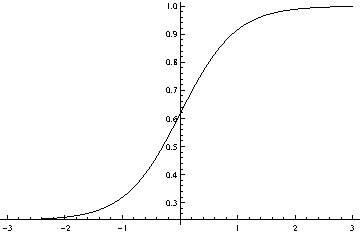
\includegraphics[width=7cm,height=4cm]{NURE2014_fig1.png}
\end{center}
\end{frame}

\begin{frame}
\frametitle{Simulated and Actual Score Distributions}
When each item is simulated and the scores added, a discrete distribution of scaled scores is generated with a histogram similar to this:
\par\vspace{0.3 cm}
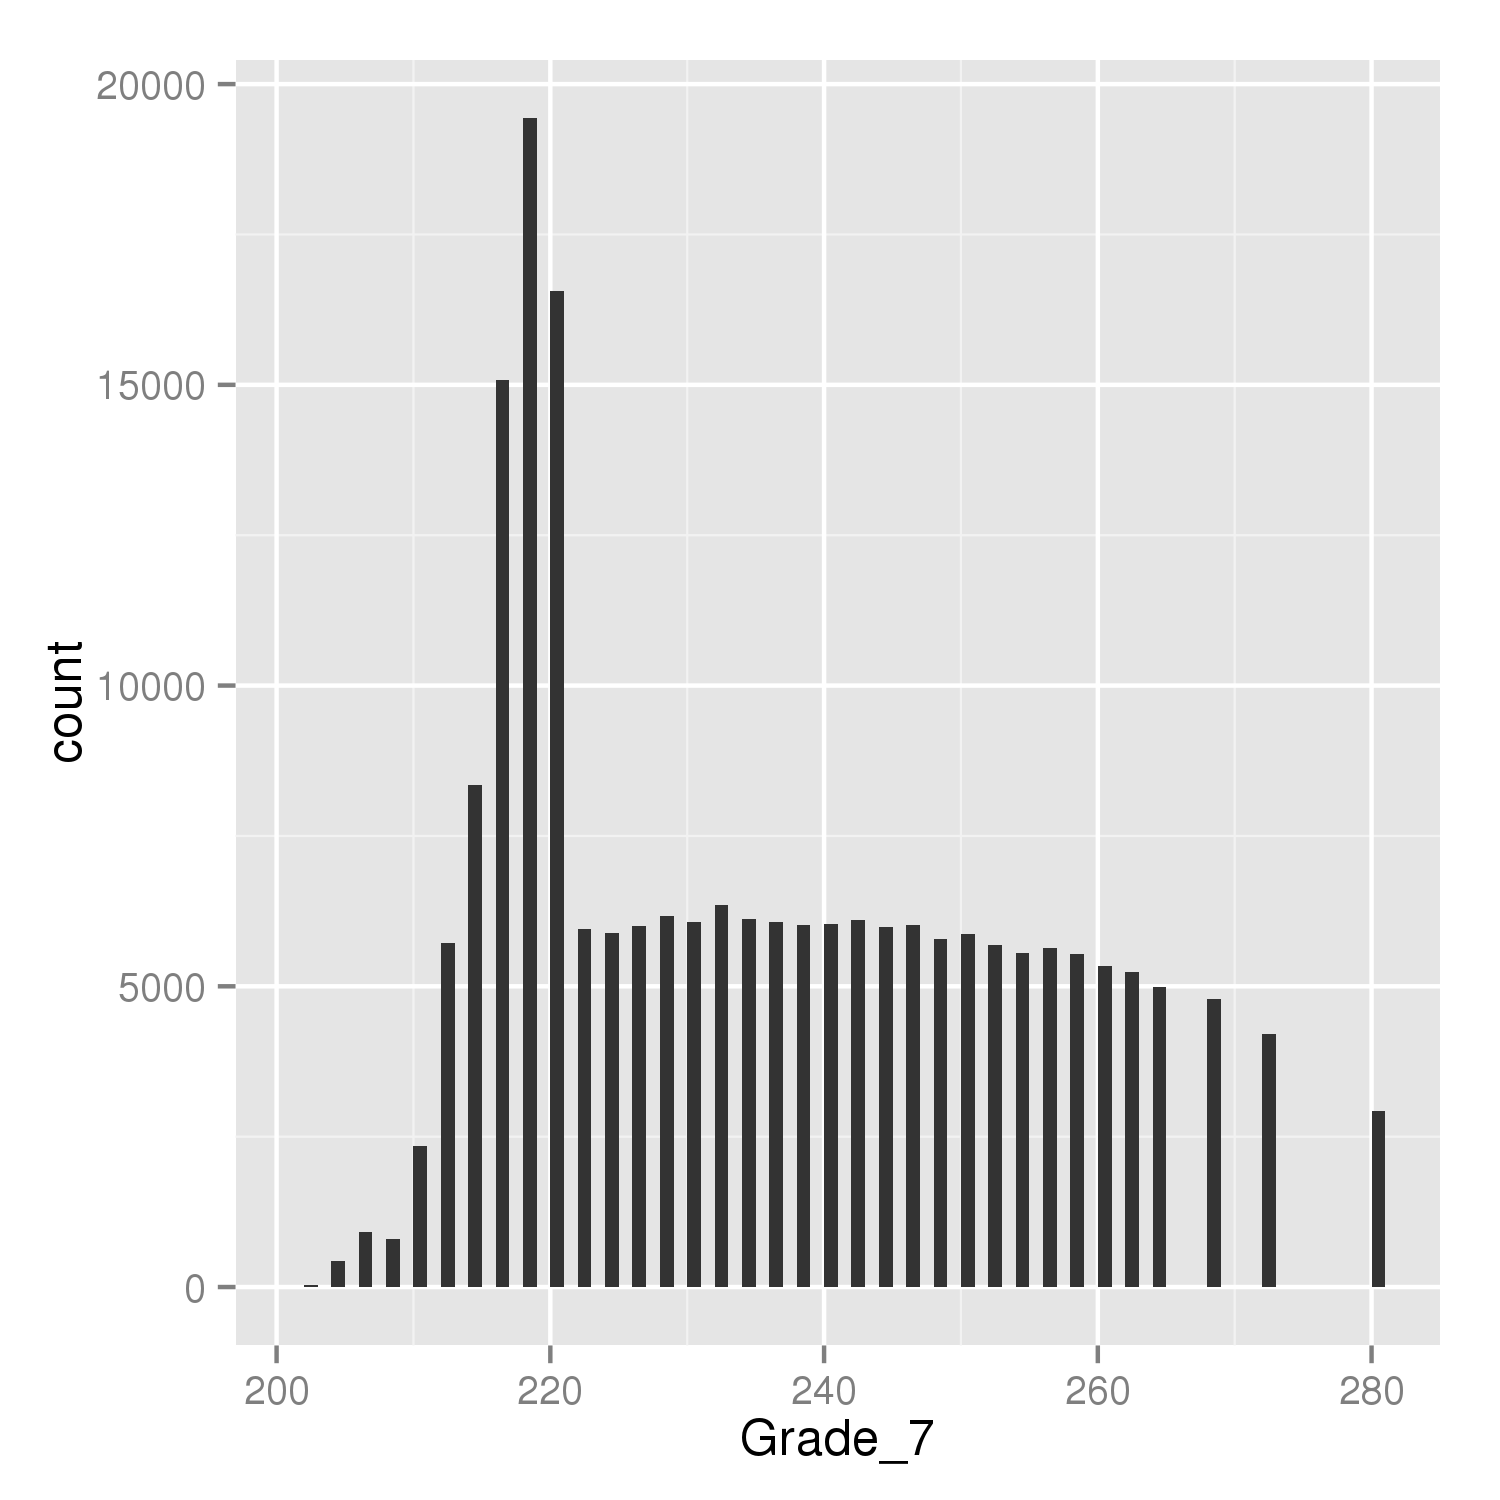
\includegraphics[width=7cm,height=5cm]{hist_Grade7.png}
\par\vspace{0.1 cm}
The IRT-based generating process reproduced the cumulative distributions well and kept the discrete character of the scores.
\end{frame}

\begin{frame}
\frametitle{Simulated and Actual Score Distributions}
The scaled scores are usually presented as a continuous graph rather than a histogram:
\par\vspace{0.3 cm}
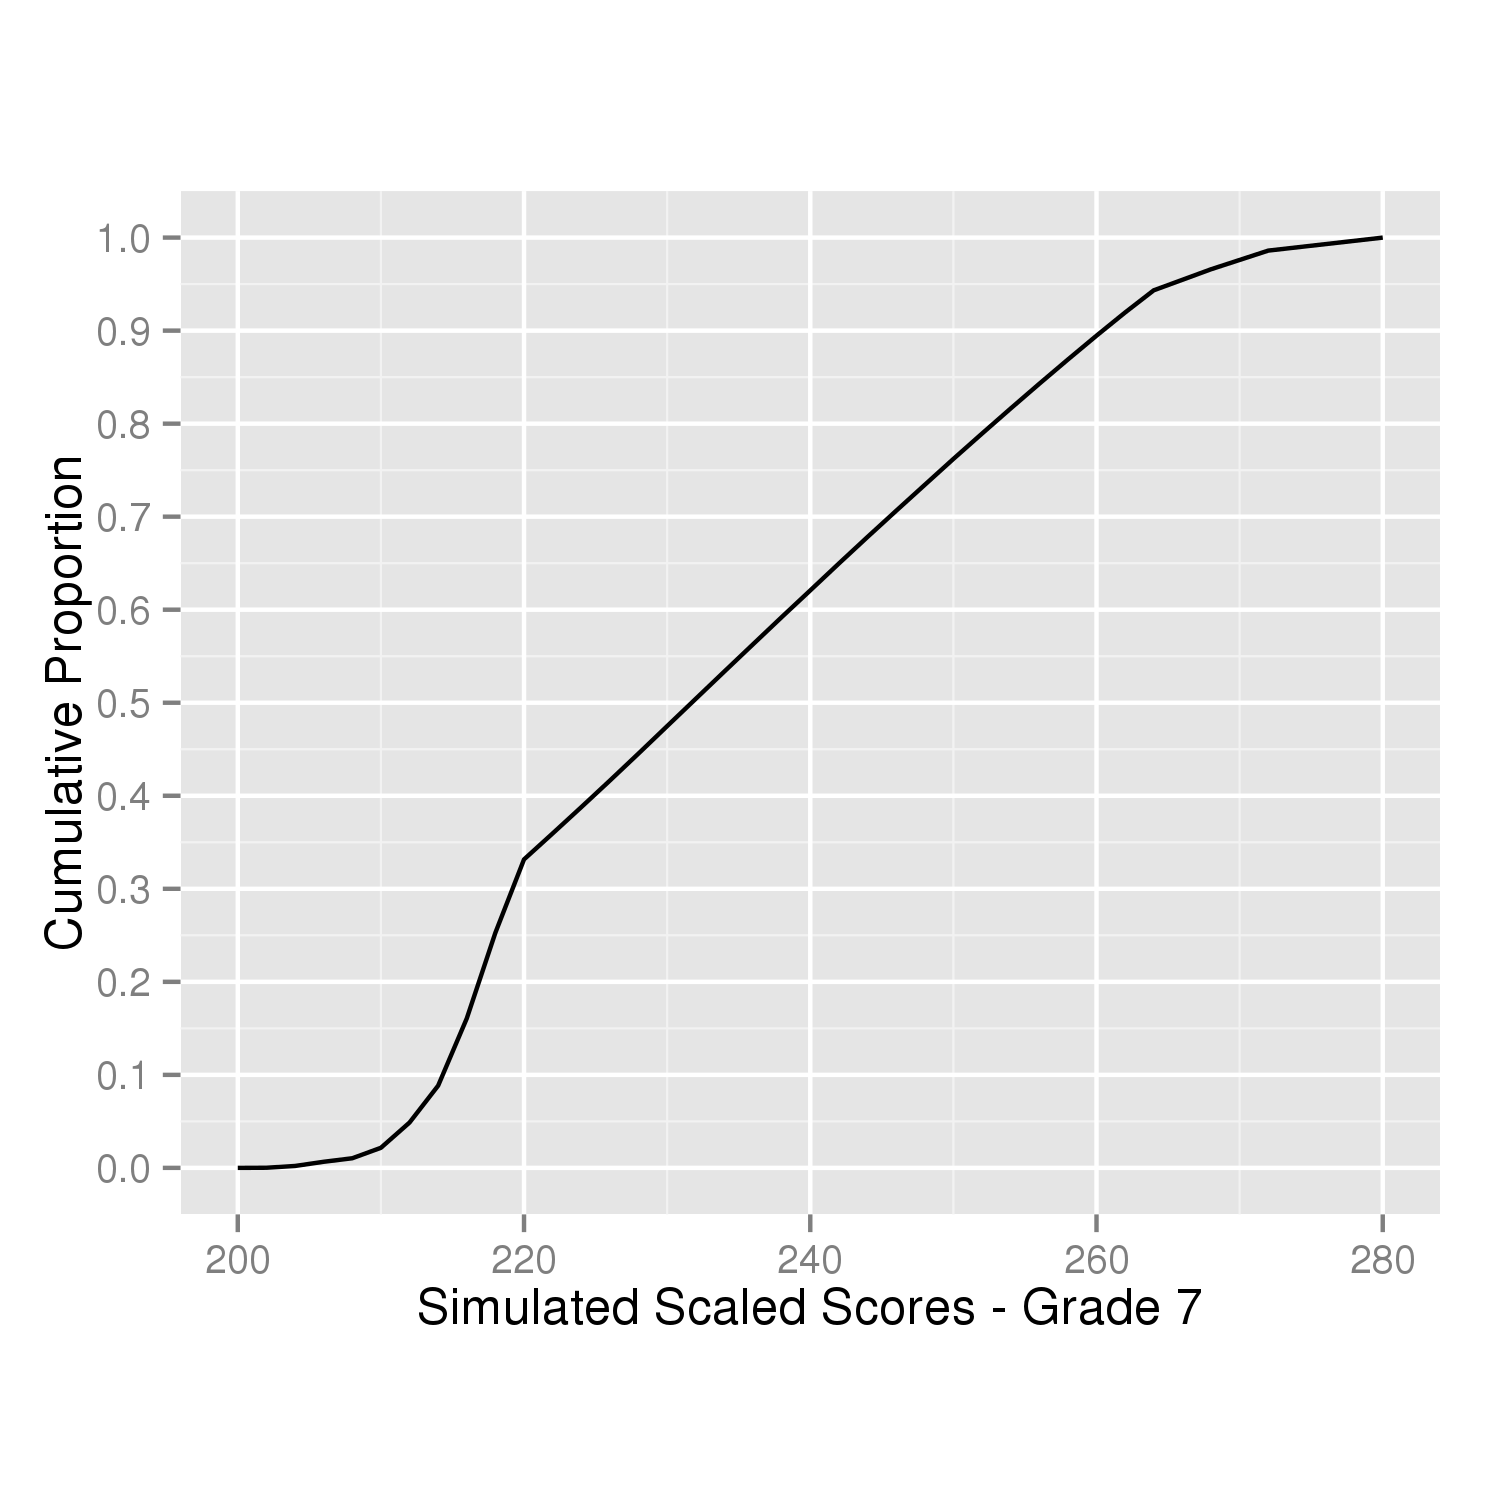
\includegraphics[width=7cm,height=5cm]{grade7sim.png}
\end{frame}
\begin{frame}

\frametitle{Simulated and Actual Score Distributions}
The cumulative distribution graph for the simulated scaled scores closely resembles that of the actual scores published by MCAS:
\par\vspace{0.3 cm}
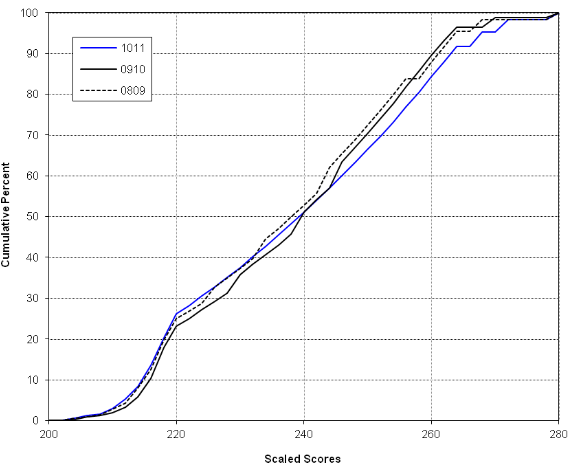
\includegraphics[width=7cm,height=5cm]{grade7.png}
\end{frame}

\begin{frame}
\frametitle{Purpose of Simulations}
The use of simulated rather than actual MCAS scores makes it possible to:
\par\vspace{0.5 cm}
\begin{itemize}  
\item  Simulate repeated administration of the MCAS to the same student to estimate measurement error.
\item  Simulate using the same test for multiple years, creating a vertical scale.
\end{itemize}
\end{frame}
\end{document}
